\chapter{The Future}

\section{Future of Networking}

\subsection{Faster Hardware}
Use of ASICs (Application Specific Integrated Circuits) to make faster network switches.
\\
\\ One example of this is Barefoot Networks (purchased by Intel in 2019). They
create high speed Ethernet ASICs with a programmable pipeline (using a language called P4).
Their Tofino 2 switch can handle $12.8 \ Tbps$.
\\
\\ Many other companies such as Cisco also vend ASIC based network gear.
\\
\\ Another consideration is using light as a medium for secure communications, better fibre optics.

\subsection{Faster Wireless}
\href{https://kumunetworks.com/}{Kumu Networks} have developed programmable filters to
allow wireless devices to cancel out their own transmissions. This allows full-duplex
wireless as wireless devices can receive and transmit simultaneously on a single channel.
\\
\\ Scientists in Japan and Germany have developed on \href{https://spectrum.ieee.org/recordsetting-terahertz-transmitters}{terahertz transmitters} ($1.1 \ THz$) allowing for far higher data transfer speeds

\subsection{Legislation}
Net-Neutrality laws in the USA (though can affect the entire world as they affect internet infrastructure) allow ISPs
to be selective about services provided for content on the internet (e.g slowing down a competitor's website,
offering special packages allowing access to a limited number of sites).

\subsection{Wireless Mesh}
Allowing many wireless devices to form a mesh network. For example \href{https://meraki.cisco.com/en-uk/}{Cisco Meraki}
allows for networks to self-heal when parts of the network (e.g switches) fail, by rerouting data wirelessly.

\subsection{Software Defined Networking (SDN) and Network FUnctions Virtualization (NFV))}
A network architecture where applications and services are abstracted from the network infrastructure \& control.
\\
\\ Useful for containerization, and being developed by Nicira (now owned by VMWare), Cisco and others.
\begin{center}
    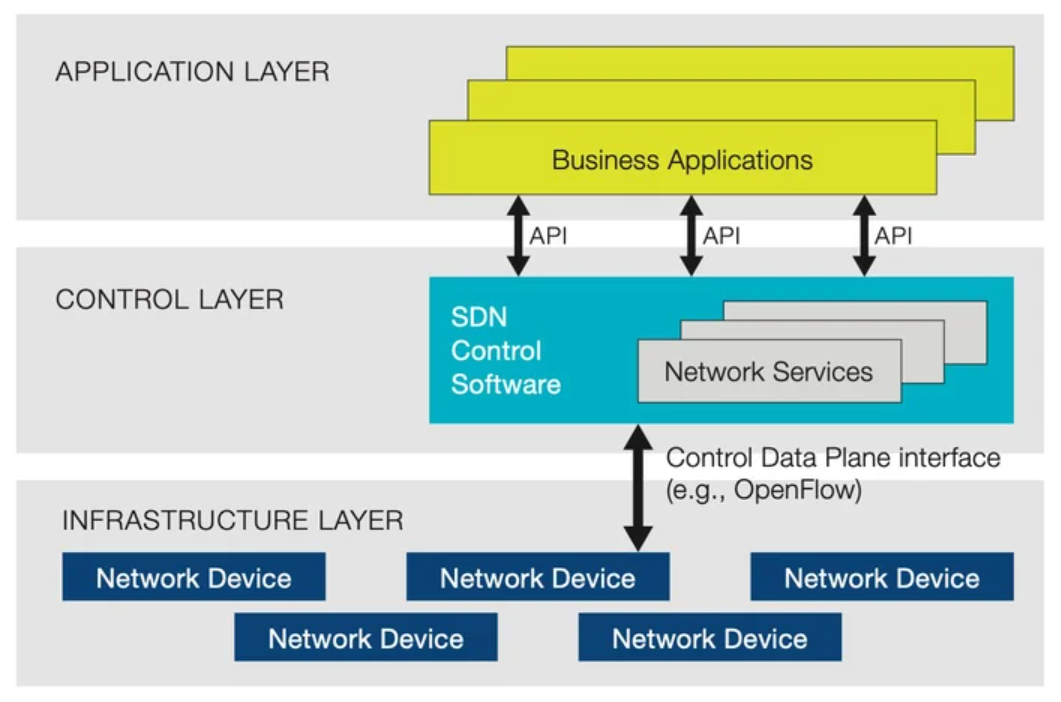
\includegraphics[width=0.8\textwidth]{the_future/images/sdx central SDN}
\end{center}

\subsection{Web-Decentralisation}
The internet has become more centralised around large \keyword{CDNs} such as Amazon's, Google's, and around few large services (e.g facebook, youtube).
\\
\\ This is bad for reliability (if a few backbones go down, large services disappear).
\\
\\ New protocols such as \href{https://ipfs.io/}{IPFS} intend to resolve this.
\\
\\ Many users can aide decentralisation by using their own domains, storage (e.g instead of google drive, dropbox) and their own hosting services.

\subsection{Jobs in Networking}
\termdef{Network Engineer}{
    An engineer specialising in manageing computer networks, typically with expertise in:
    \compitem{
        \item Infrastructure
        \item Virtualisation (e.g VLANs)
        \item Servers
        \item Switches
        \item Firewalls
        \item Meraki
        \item WatchDog
    }
    Some certifications used include:
    \compitem{
        \bullpara{CCNP}{\href{https://www.cisco.com/c/en/us/training-events/training-certifications/certifications/professional.html}{Professional-level certification by cisco}.}
        \bullpara{CISSP}{Certified Information Systems Security Professional, a cybersecurity competency certification.}
        \bullpara{RHCE}{\href{https://www.redhat.com/en/services/certification/rhce}{Red Hat Certified Engineer}}
    }
}
